\section{Problem 1}
\textit{ Using the method of moments code from Agilent ADS simulate a Yagi-Uda antenna that has a gain of at least 6 dBi at 850 Mhz.}\\

We implemented the same antenna design as implemented in CST in mm7. The designed Yagi antenna in ADS is giving a gain patten as shown in \figref{fig:3d_ADS}. The polar plot is shown in \figref{fig:ADS_pattern} and in \figref{fig:ADS_cart_pattern} the Cartesian version is also presented. Note that the plot here shows a very large gain, this is not true but a normalization issue with ADS. The gain pattern when compared CST is similar. In \figref{fig:ADS_S11} the matching (S11) is shown. 

\begin{figure}[!h]
  \centering
  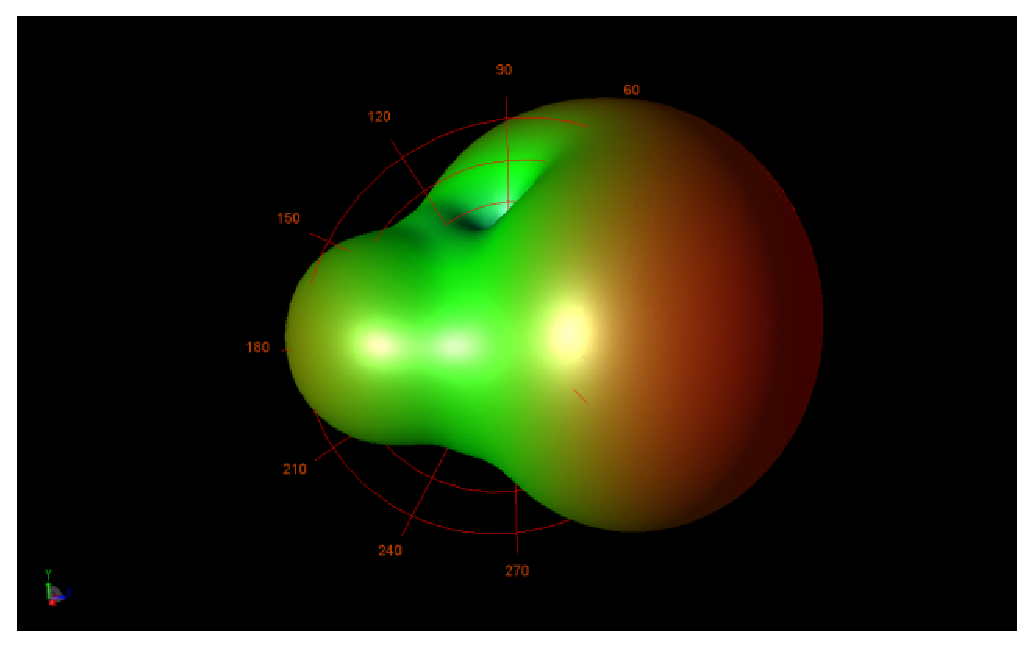
\includegraphics[width=11cm]{3d_ADS.eps}
  \caption{Figure showing the 3D gain patten of the ADS designed antenna.}
  \label{fig:3d_ADS}
\end{figure}

\begin{figure}[!h]
  \centering
  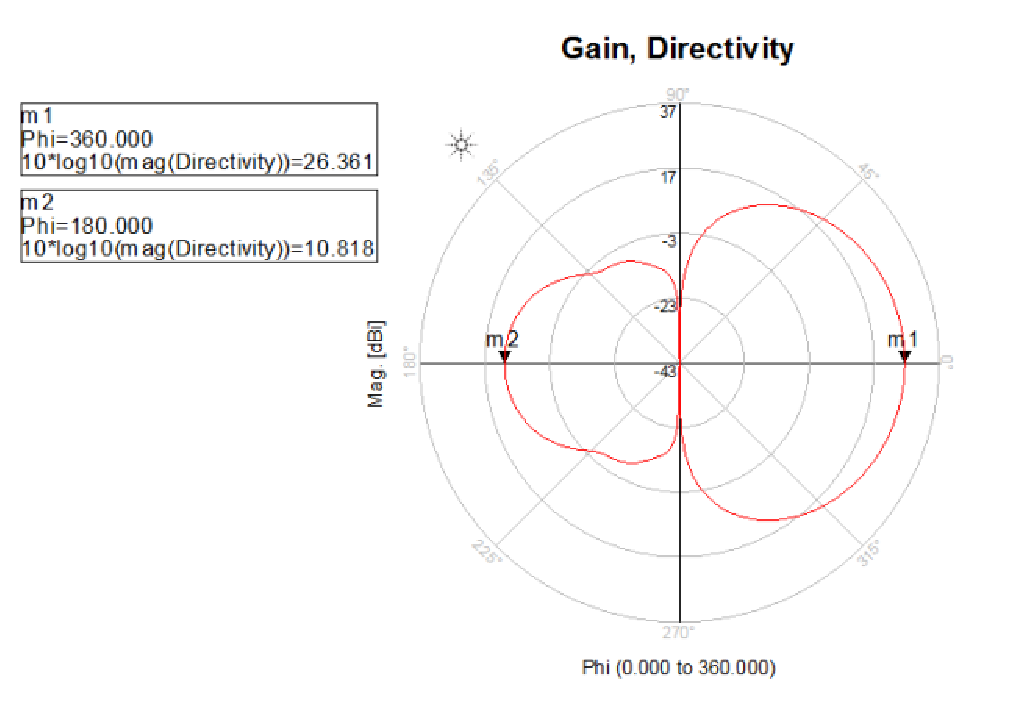
\includegraphics[width=11cm]{ADS_pattern.eps}
  \caption{Figure showing the polar gain patten of the ADS designed antenna.}
  \label{fig:ADS_pattern}
\end{figure}

\begin{figure}[!h]
  \centering
  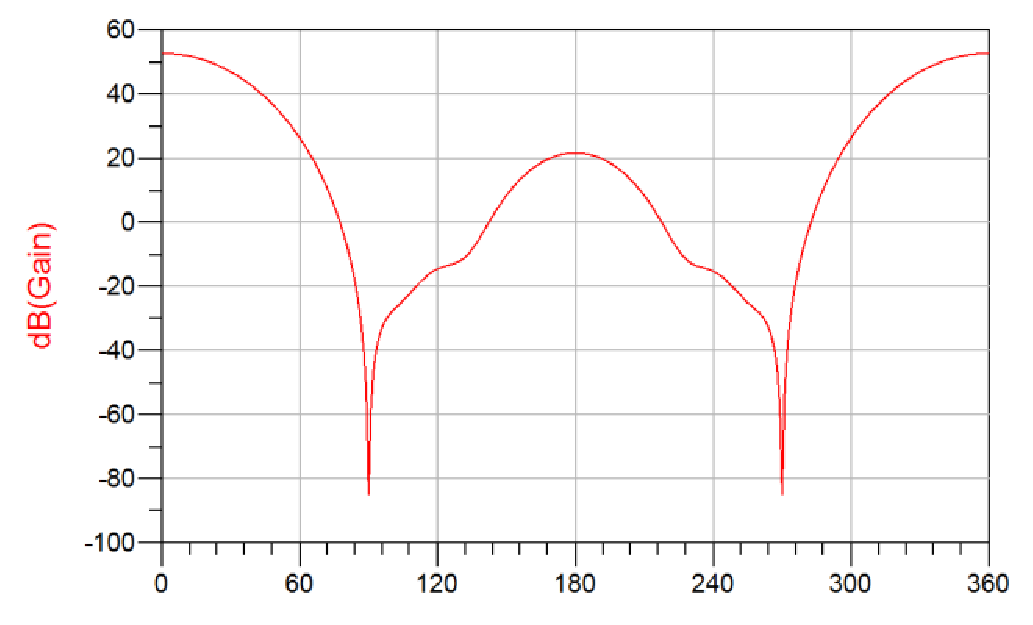
\includegraphics[width=11cm]{ADS_cart_pattern.eps}
  \caption{Figure showing the Cartesian gain patten for the ADS designed antenna.}
  \label{fig:ADS_cart_pattern}
\end{figure}

\begin{figure}[!h]
  \centering
  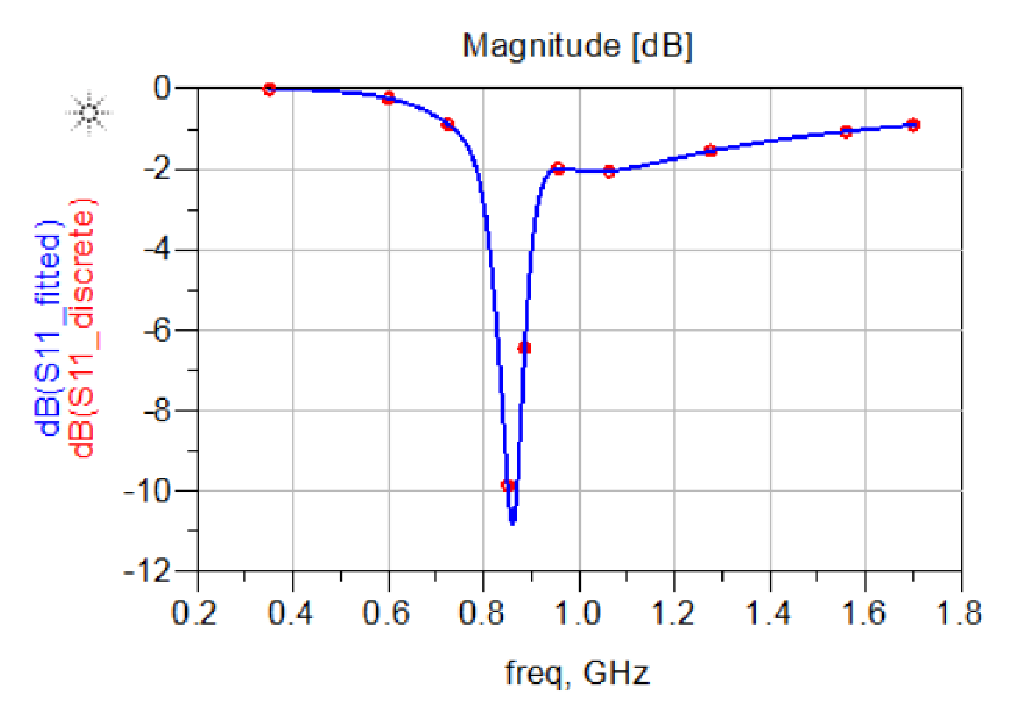
\includegraphics[width=11cm]{ADS_S11.eps}
  \caption{Figure showing the matching (S11) for the ADS designed antenna.}
  \label{fig:ADS_S11}
\end{figure}

